\documentclass[paper=a4, fontsize=11pt]{article} % A4 paper and 11pt font size

% for pandoc conversion
\providecommand{\tightlist}{%
  \setlength{\itemsep}{0pt}\setlength{\parskip}{0pt}}

\usepackage[export]{adjustbox}
\usepackage{subcaption}
\usepackage{wrapfig}
\usepackage[margin=1in]{geometry}
%\usepackage[T1]{fontenc} % Use 8-bit encoding that has 256 glyphs
%\usepackage{fourier} % Use the Adobe Utopia font for the document - comment this line to return to the LaTeX default
\usepackage[english]{babel} % English language/hyphenation
\usepackage{mathtools,amsfonts,amsthm} % Math packages
\usepackage{graphicx}
\usepackage{listings}
\usepackage{color}
\definecolor{mygreen}{rgb}{0,0.5,0}
\definecolor{mygray}{rgb}{0.5,0.5,0.5}
\definecolor{mymauve}{rgb}{0.58,0,0.82}
\usepackage{multicol}

% including packages for hyperlink
\usepackage{hyperref}
\hypersetup{
	colorlinks=true,
	linkcolor=blue,
	filecolor=magenta,      
	urlcolor=cyan,
	citecolor=cyan,
}

\usepackage{minted}
\usepackage{xcolor}
\definecolor{LightGray}{gray}{0.95}

\usepackage{url}
\usepackage{titlesec}
\titleformat{\paragraph}
{\normalfont\normalsize\bfseries}{\theparagraph}{1em}{}
\titlespacing*{\paragraph}
{0pt}{3.25ex plus 1ex minus .2ex}{1.5ex plus .2ex}
\setcounter{secnumdepth}{4}

\lstset{ 
basicstyle=\small,
language=[Sharp]C,
commentstyle=\color{mygreen},
frame=single,
numbers=left,
%numbersep=5pt,
%title=\lstname ,
captionpos=b,
breaklines, 
caption=\lstname}

\usepackage{float}
\usepackage{placeins}


\usepackage{hyperref}

\usepackage{fancyhdr} % Custom headers and footers
\fancyhead[C]{} % No page header - if you want one, create it in the same way as the footers below
\fancyhead[L]{ARRP -- MUEEC}
\fancyhead[R]{Intro to Motors}
\fancyfoot[L]{} % Empty left footer
\fancyfoot[C]{\thepage} % Empty center footer
\fancyfoot[R]{} % Page numbering for right footer
\setlength{\headheight}{15pt} % Customize the height of the header

\numberwithin{equation}{section} % Number equations within sections (i.e. 1.1, 1.2, 2.1, 2.2 instead of 1, 2, 3, 4)
\numberwithin{figure}{section} % Number figures within sections (i.e. 1.1, 1.2, 2.1, 2.2 instead of 1, 2, 3, 4)
\numberwithin{table}{section} % Number tables within sections (i.e. 1.1, 1.2, 2.1, 2.2 instead of 1, 2, 3, 4)

\setlength\parindent{0pt} % Removes all indentation from paragraphs - comment this line for an assignment with lots of text

% including packages for hyperlink
\usepackage{hyperref}
\hypersetup{
	colorlinks=true,
	linkcolor=blue,
	filecolor=magenta,      
	urlcolor=cyan,
	citecolor=cyan,
}

%----------------------------------------------------------------------------------------
%	TITLE SECTION
%----------------------------------------------------------------------------------------

\newcommand{\horrule}[1]{\rule{\linewidth}{#1}} % Create horizontal rule command with 1 argument of height

\begin{document}
%----------------------------------------------------------------------------------------

\begin{titlepage}
	\begin{center}
		\begin{LARGE}
			Melbourne University Electrical Engineering Club\\
		\end{LARGE}
		\hrulefill\\
		\vfill
		\begin{Huge}
			\textbf{Intro to Motors} \\
		\end{Huge}
		\begin{large}
			\vfill
			
			\begin{tabular}{c}
				Jun Yi Van\\
				Andrew Huang\\
				Steven Lee
			\end{tabular}
		\end{large}
	\end{center}
	\vfill
	\begin{minipage}{\linewidth}
		
\includegraphics[height=2cm]{./mueec_logo.png}
		\hfill
		
\includegraphics[height=2cm]{./arrp_logo.png}
	\end{minipage}
\end{titlepage}

\newpage

\pagestyle{fancy} % Makes all pages in the document conform to the custom headers and footers
\textbf{Disclaimer}: This is not a comprehensive write-up regarding the
topic of electric motors. Please consult additional sources in
literature for complete details.

\hypertarget{general-terminology}{%
\section{General Terminology}\label{general-terminology}}

% Add to the general terminology as the write-up continues.

\begin{itemize}
\tightlist
\item
  RPM: revolution per minute.
\item
  Brushed motors: commutation carried out using brushes (mechanically).
  Brushes are the component that provide stationary electrical contact
  to the moving commutator conducting segments.
\item
  Brushless motors: physical commutator is not used, instead the control
  electronics switching the DC current in the stator coils.
\end{itemize}

\hypertarget{motors}{%
\section{Motors}\label{motors}}

In this section, we will go over various types of motors, how they work
and how we can use them in your future projects.

\hypertarget{dc-motors}{%
\subsection{DC Motors}\label{dc-motors}}

While there are many different sub-categories for DC motors, we will
focus on one main type for the purpose of this tutorial/demonstration.

\hypertarget{geared-motors}{%
\subsubsection{Geared Motors}\label{geared-motors}}

Geared motors are one type of DC motors where additional gearing is
installed to increase/decrease the output torque of the motor. If we
start off with a basic motor construction, we can add additional gearing
to increase its output torque while reducing its operational speed.

For example, if we have an electric motor that drives a 10-tooth gear
that meshes with a 50-tooth gear, then a reduction of 5:1 is achieved
(50/10 = 5).

If that electric motor runs at 1,000 rpm, then the gearbox will reduce
the speed by 5 times to 200 rpm. If the motor torque is 10 Nm, then the
gearbox increases this torque by a factor of 5 to 50 Nm.

Note that the efficiency losses have not yet been taken into account, so
the actual performance would be slightly lower.

For your application, it will be important to consider the required
torque for driving a fully loaded robot. If your motor has really high
rpm but really low torque, then the robot may not be able to move at
all.

\hypertarget{encoder}{%
\subsubsection{Encoder}\label{encoder}}

In order to better control our motors, we need a way to know how much
the motor shaft has turned. That is, we need to find the displacement of
the motors. This is where encoders come in.

\textbf{Encoders are position measurement devices and can be categorised
as one of the following.}

\begin{enumerate}
\def\labelenumi{\arabic{enumi}.}
\tightlist
\item
  Incremental Encoder

  \begin{itemize}
  \tightlist
  \item
    Simpler mechanism
  \item
    Tracks only relative displacement
  \item
    Cheaper
  \end{itemize}
\item
  Absolute Encoder

  \begin{itemize}
  \tightlist
  \item
    More complex mechanism
  \item
    Tracks absolute displacement
  \item
    More expensive
  \end{itemize}
\end{enumerate}

\hypertarget{incremental-encoder}{%
\paragraph{Incremental Encoder}\label{incremental-encoder}}

A basic incremental encoder works on a principle similar to a
opto-electronic switch. When the light source passes through a gap on
the disk, the signal goes from low to high and then we know that the
disk has moved a certain amount.

If you start looking for encoders or motors with encodes, you will
eventually come across the term \textbf{Quadrature Encoder}. Quadrature
encoder is a type of encoder with two specific channels.

\begin{itemize}
\tightlist
\item
  Channel A
\item
  Channel B
\end{itemize}

\begin{figure}[H]
\centering
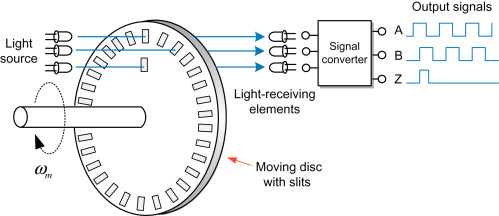
\includegraphics[width = 0.8 \textwidth]{2019-08-05-21-00-32.png}
\caption{Quadrature Encoder Diagram \\
Image Source:
\href{https://www.sciencedirect.com/topics/engineering/incremental-encoder}{Science
Direct}.}
\end{figure}

These channels are coded in so that they are 90 degrees out of phase,
which provide the ability for direction sensing and higher encoder
resolution.

Sometimes quadrature encoders come with a Channel Z, which provides a
signal when a full revolution is completed.

\hypertarget{absolute-encoder}{%
\paragraph{Absolute Encoder}\label{absolute-encoder}}

As the name suggests, an absolute encoder provides us the absolute
position of the motor, so that we can tell exactly how the motor shaft
and the attached object is oriented. The absolute encoder uses a gray
encoding setup to keep track of the current shaft position.

The accuracy of the absolute encoder depends on the number of
bits/channels available. For example, an absolute encoder with 10
channels, cna distinguish the absolute orientation of a joint up to a
resolution of

\begin{equation*}
    360 \div 2^{10} = 0.3515625 \text{ degrees}
\end{equation*}

In practice, you do not always have to go for the absolute encoder. Instead, if you keep track of your initial condition and setup the required book-keeping routine, an incremental encoder can be sufficient for most tasks. For more information about Incremental Encoder, please see the webpage on \href{https://www.sciencedirect.com/topics/engineering/incremental-encoder}{Science
Direct}.

\hypertarget{motor-controllers-h-bridges}{%
\subsubsection{Motor Controllers
(H-bridges)}\label{motor-controllers-h-bridges}}

Common microcontrollers such as the Arduino Uno is only capable of
outputing a small amount of current, so we are not able to drive the
motor directly (unless we have a really small motor).

Most commonly these days, motor drivers use a H-bridge to DC motor.

\begin{figure}[H]
    \centering
    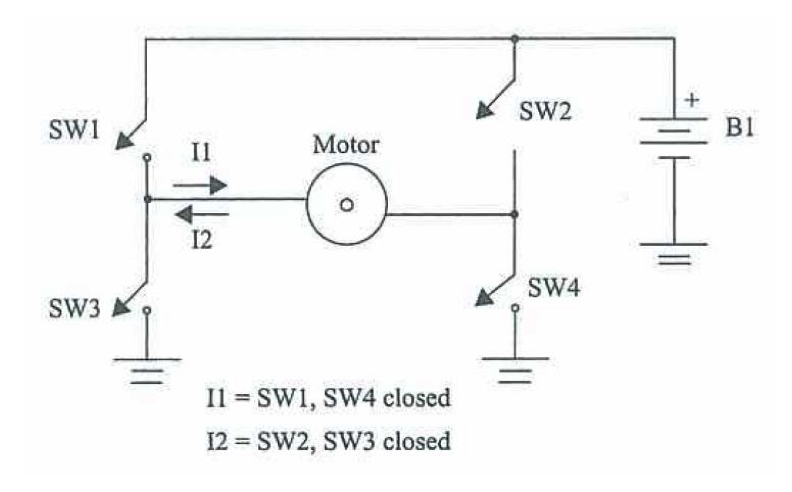
\includegraphics[width = 0.6 \textwidth]{2019-08-05-21-37-19.png}
    \caption{H-Bridge Schematic \\
    Image Source: Mechatronics
Systems Design Lecture 11}
    \label{fig:h_bridge}
\end{figure}


From the h-bridge schematic above, we can see that:

\begin{itemize}
\tightlist
\item
  When switch 1 and switch 4 are closed, current flows in the I1
  direction.
\item
  When switch 2 and switch 3 are closed, current flows in the I2
  direction.
\end{itemize}

Depending on the specific configuration of the switches, we can
determine the direction of the motor movement.

\hypertarget{pwm-driving-signal}{%
\subsubsection{PWM Driving Signal}\label{pwm-driving-signal}}

With a H-bridge, we would commonly use a PWM (Pulse Width Modulation) signal to drive the motor. PWM is a more power efficient way that uses square voltage pulses to drive the motor. For this to work, we would need to specify the desired frequency and duty cycle.

On the
\href{https://knowledge.ni.com/KnowledgeArticleDetails?id=kA00Z0000019OkFSAU\&l=en-AU}{National
Instruments PWM Page}, they provide a good overview of what PWM is and
how to use it. In summary, the frequency required depends on the
application and the response time of the system. From the NI PWM page:

\begin{itemize}
\tightlist
\item
  Heating elements or systems with slow response times: 10-100 Hz or
  higher
\item
  DC electric motors: 5-10 kHz or higher
\item
  Power supplies or audio amplifiers: 20-200 kHz or higher
\end{itemize}

The duty cycle parameter is used determine how fast we want to drive the
motor. A 25\% duty cycle means that we will generate a square wave with
25\% high and 75\% low.

\begin{figure}[H]
\centering
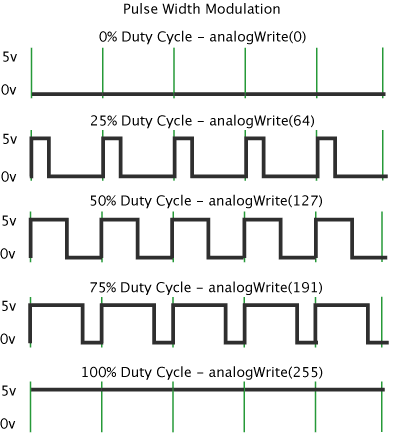
\includegraphics[width = 0.5 \textwidth]{2019-08-05-22-03-08.png}
\caption{Duty Cycle \\
Image Source: \href{https://www.arduino.cc/en/Tutorial/PWM}{Arduino PWM Tutorial Page}}
\end{figure}

Notice that the PWM signal can be generated using the
\texttt{analogWrite()} function in Arduino. Please see the Arduino
\href{https://www.arduino.cc/en/Tutorial/PWM}{PWM Tutorial Page} for
more details.

\hypertarget{servo-motors}{%
\subsection{Servo Motors}\label{servo-motors}}

See example from Arduino 202 Tutorial.

\hypertarget{stepper-motors}{%
\subsection{Stepper Motors}\label{stepper-motors}}
There are two basic types of stepper motors.

\begin{enumerate}
    \item Permanent Magnet (PM)
    \item Variable Reluctance (VR) with non-magnetised soft-iron rotors
\end{enumerate}

The stepper motor resolution depends on whether it uses:

\begin{itemize}
    \item Full-stepping
    \item Half-stepping
    \item Micro-stepping
\end{itemize}

Full-stepping is when only one phase is activated at any given time. Half-stepping is when phases are activated in alternating routine between one-phase and two-phase. Micro-stepping is when the phases are electronically controlled so that the rotors can move in very small steps.

\hypertarget{ac-motors}{%
\subsection{AC Motors}\label{ac-motors}}

As the name suggests, AC motors make use of alternating current for operation. It is most likely not used for your small scale robotics/mechatronics project, but it is still an important mention as it is widely used in the heavy industries. For example, they are used in dryers, washing machines and fans.

\begin{enumerate}
\def\labelenumi{\arabic{enumi}.}
\tightlist
\item
  This \href{https://www.youtube.com/watch?v=AQqyGNOP_3o}{video}
  provides a great overview on how an AC Induction Motor works, they are
  also known as asynchronous motors.
\item
  This \href{https://www.youtube.com/watch?v=Vk2jDXxZIhs}{video}
  provides a good overview on how a Synchronous Motor works, which is
  another type of AC motor.
\end{enumerate}

% \hypertarget{motor-selection}{%
% \section{Motor Selection}\label{motor-selection}}

% Consult Andrew for further write-up.

% \begin{itemize}
% \tightlist
% \item
%   Finding coefficient of friction
% \item
%   Incline test
% \item
%   Research and finding engineering papers
% \item
%   How to find torque needed
% \item
%   Torque RPM Curve
% \end{itemize}


% ---

% \hypertarget{steering}{%
% \section{Steering}\label{steering}}

% \begin{itemize}
% \tightlist
% \item
%   Different types of steering, see NI-1 folder for the different types
%   of steering investigated.
% \end{itemize}

% \hypertarget{platform-experiment}{%
% \section{Platform Experiment}\label{platform-experiment}}

% \begin{itemize}
% \tightlist
% \item
%   For maximum re-usability, can demon using the NI-1 robot from last year. But may need to spend some time on restoration and testing.
% \end{itemize}

% If time permits, prepare 3 carts

\begin{enumerate}
\def\labelenumi{\arabic{enumi}.}
\tightlist
\item
  DC Motors
\item
  Servo Motors (does this even make sense?)
\item
  Stepper Motors
\end{enumerate}


\newpage

\section{Running A DC Motor with H-Bridge}
Here, we will be going through how to setup a simple DC motor and control it with a Pololu VNH5019A Motor Driver.

\subsection{Wiring Guide}

\begin{figure}[H]
    \centering
    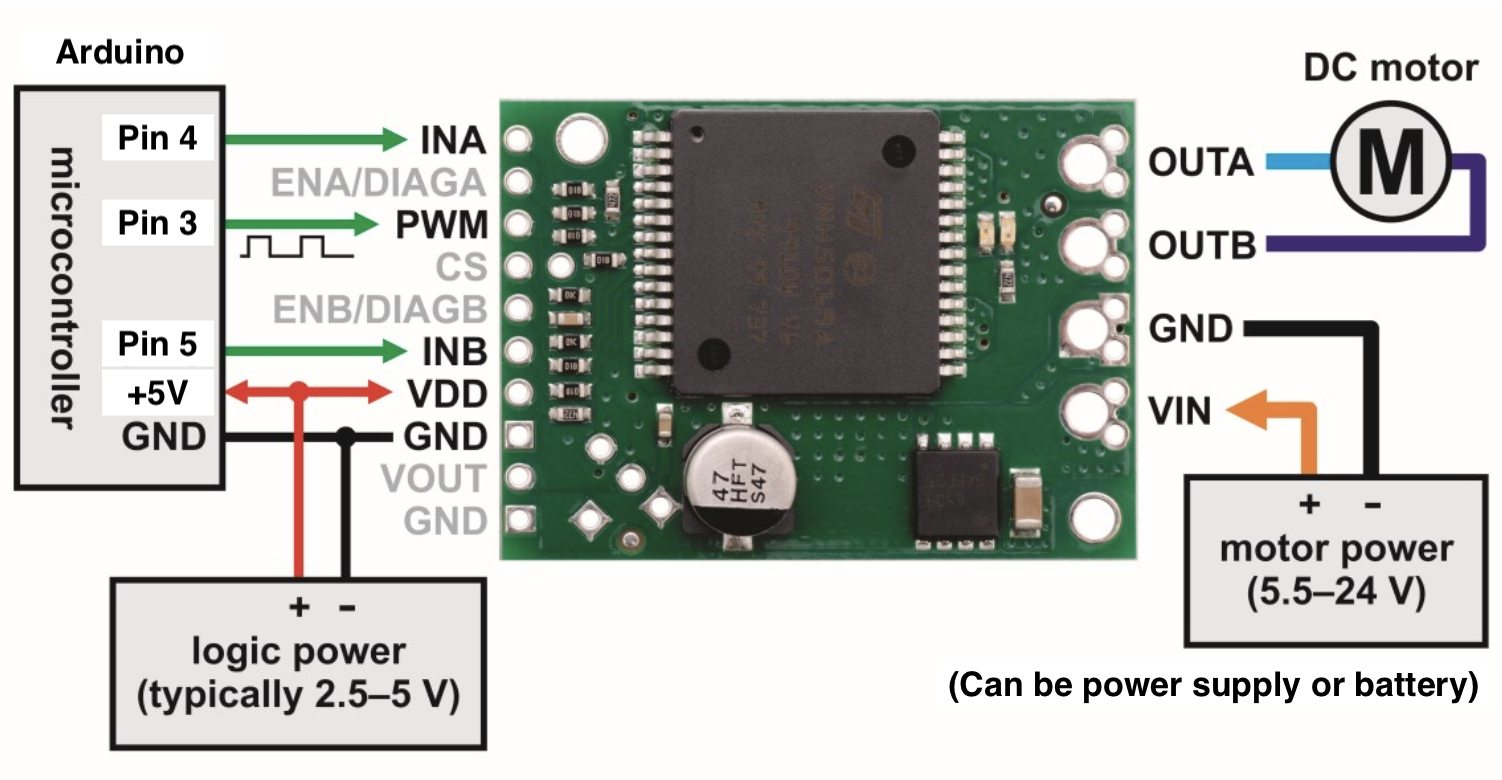
\includegraphics[width = 0.8 \textwidth]{motor_driver_wiring.png}
    \caption{Motor Driver Wiring}
    \label{fig:motor_driver_wiring}
\end{figure}

Note that for the purpose of this demonstration, we will only need to connect 5 pins to the Arduino Uno. This involves connecting the INA and INB to any of the available digital pins, in this case we have arbitrarily chosen Pin 4 and Pin 5 respectively. Similarly, PWM pin can be plugged into any of the digital pins which support PWM output from the Arduino.

\subsection{Codes for Arduino}

\inputminted[
frame=lines,
framesep=2mm,
baselinestretch=1.2,
bgcolor=LightGray,
fontsize=\footnotesize,
linenos
]{cpp}{MyDcMotorDriver.ino}

Here, we will briefly go over and justify the values which we have chosen for INA and INB. From figure \ref{fig:vnh5019a_pg14}, we can see the table of values from the original VNH5019A Datasheet, which you can open by clicking \href{https://www.pololu.com/file/0J504/vnh5019.pdf}{here}. 

\begin{itemize}
    \item By setting INA = 1 and INB = 0, we are telling the motor driver to run the motor in clockwise direction.
    \item If we set INA = 0 and INB = 1, then the motor will run in the counter-clockwise direction.
    \item Note that the motor rotation direction can also be inverted by inter-changing the pins OUTA and OUTB.
\end{itemize}
 

\begin{figure}[H]
    \centering
    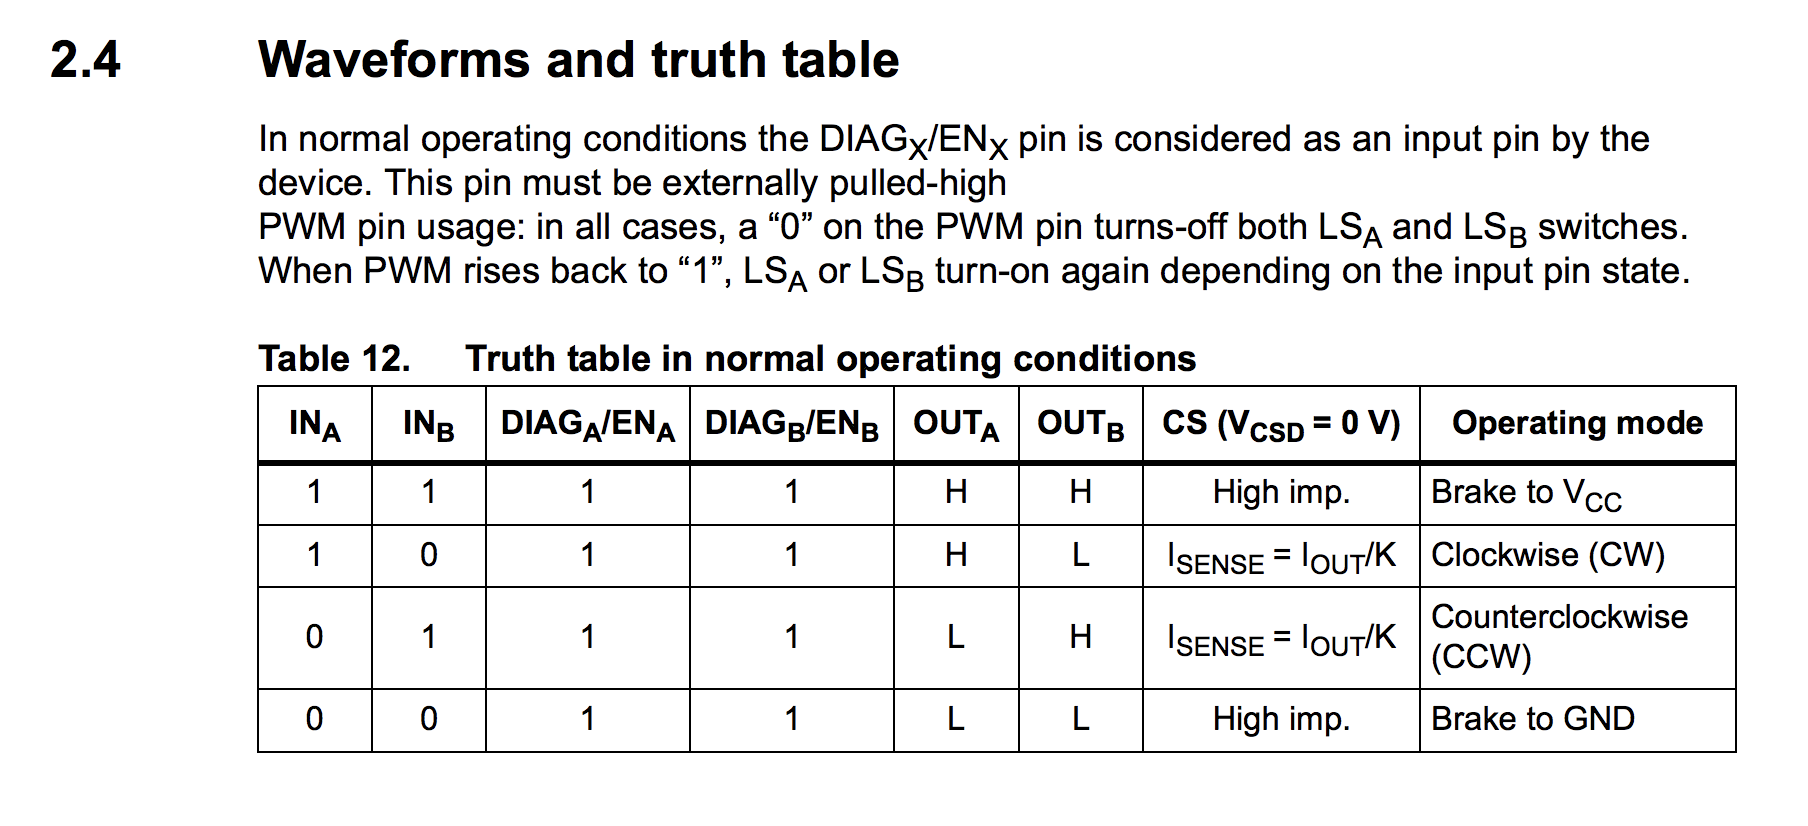
\includegraphics[width = 0.9 \textwidth]{vnh5019a_pg14.png}
    \caption{VNH5019A Datasheet Page 14 Snapshot}
    \label{fig:vnh5019a_pg14}
\end{figure}





% 1. go over how to wire everything
% 2. list the codes for arduino uno
% 3. explain the codes and mention page 14 of the motor driver data sheet
% 4. check with Jeremy to see how many actual demo 

\newpage

\section{Motor Selection}
This section is based on this guide\footnote{\url{https://www.robotshop.com/community/blog/show/drive-motor-sizing-tutorial}}.\\

Main use of motors is to convert electrical energy or signals to mechanical energy in terms of movement. Thus, proper selection of motor torque is required to ensure proper mechanical movement.\\

One of the big uses of motors is to provide torque to power wheels for motion. A method of calculating the required torque is based on the friction provided between the wheels and surface.\\

\begin{minipage}{\textwidth}
	\centering
	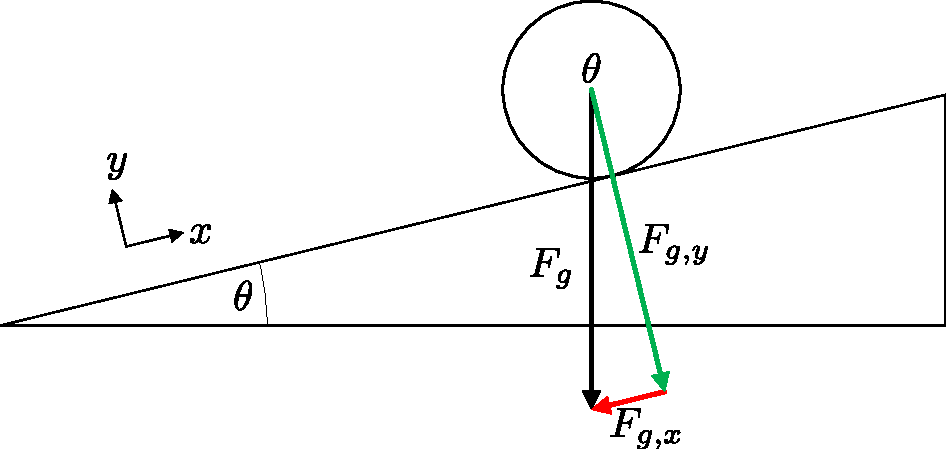
\includegraphics[width=0.5\textwidth]{./ramps/ramp1.pdf}
	\captionof{figure}{Force decomposition}
\end{minipage}

\begin{align*}
	F_g &= mg\\
	F_{g,x} &= F_g \sin(\theta)\\
	F_{g,y} &= F_g \cos(\theta)
\end{align*}
If we now include torque on the wheel and the friction between the wheel and the ramp.\\

\begin{minipage}{\textwidth}
	\centering
	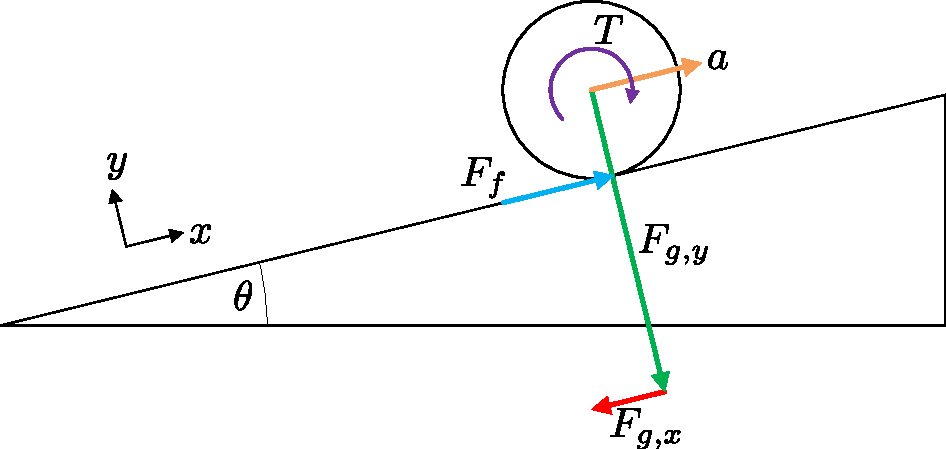
\includegraphics[width=0.5\textwidth]{./ramps/ramp2.pdf}
	\captionof{figure}{Free body diagram}
\end{minipage}
\vspace{1em}\\
Now for the wheel to be rolling without slip the point in which the wheel and ramp come into contact is static ($v = a = 0$). Thus,
\begin{equation*}
	F_f = Tr + F_{g,x}
\end{equation*}
Finally, summing all forces on the wheel,
\begin{equation*}
	\sum F_x = F_f - F_{g,x} = ma
\end{equation*}
An important thing to note, is that this all assumes a wheel rolling with no slip. Thus, there is a limit to the frictional force ($F_f \leq \mu_s F_{g,y}$) and hence the overall acceleration is also limited.
\end{document}